%\documentclass[handout]{beamer}
\documentclass[aspectratio=169]{beamer}
\usepackage{etex} % fixes new-dimension error

\usetheme{metropolis}
\usepackage{appendixnumberbeamer}

% Base colors (from metropolis theme)
\definecolor{metDarkBrown}{HTML}{604c38}
\definecolor{metDarkTeal}{HTML}{23373b}
\definecolor{metLightBrown}{HTML}{EB811B}
\definecolor{metLightGreen}{HTML}{14B03D}

 

\metroset{numbering=fraction,progressbar=frametitle}

% \setbeamercolor*{structure}{fg=blue!80!black}
\setbeamercolor*{structure}{fg=metLightGreen}

% % \definecolor{MainColour}{rgb}{0., 0.25, 0.8}
% \colorlet{MainColour}{blue!50!black}
% \colorlet{BgColour}{blue!10}
% \colorlet{BarColour}{blue!50!black}


% %\usetheme{CambridgeUS}%{Copenhagen}%{Frankfurt}%{Singapore}%{CambridgeUS}
% \usecolortheme[named=MainColour]{structure} 
% \useoutertheme[subsection=false]{miniframes}
% \useinnertheme{circles}
% %\useinnertheme[shadow=false]{rounded}
% \setbeamertemplate{blocks}[rounded][shadow=false]

% \setbeamercovered{transparent} 
% \setbeamertemplate{navigation symbols}{} %Remove navigation bar
% \setbeamertemplate{footline}[frame number] % add page number
% \setbeamercolor{postit}{fg=MainColour,bg=BgColour}
% \setbeamercolor{structure}{bg=black!10}
% %\setbeamercolor{palette primary}{use=structure,fg=red,bg=green}
% %\setbeamercolor{palette secondary}{use=structure,fg=red!75!black,bg=green}
% \setbeamercolor{palette tertiary}{use=structure,bg=BarColour,fg=white}
% %\setbeamercolor{palette quaternary}{fg=black,bg=green}
% %\setbeamercolor{normal text}{fg=black,bg=white}
% %\setbeamercolor{block title alerted}{fg=red,bg=green}
% %\setbeamercolor{block title example}{bg=black!10,fg=green}
\setbeamercolor{block body}{bg=black!5}

% \setbeamercolor{block title alerted}{bg=red!25}
% \setbeamercolor{block body alerted}{bg=red!10}

% \setbeamercolor{block title example}{bg={rgb:green,2;black,1;white,5}}
\setbeamercolor{block body example}{bg={rgb:green,2;black,1;white,20}}
\setbeamercolor{block body alerted}{bg={metLightBrown!25}}

% \setbeamertemplate{itemize item}{\color{black!10}$\blacksquare$}
\setbeamercolor{itemize item}{fg=metDarkTeal}
\setbeamercolor{itemize subitem}{fg=metDarkTeal}

\setbeamercolor{graybc}{fg=black,bg=black!10}
\newcommand{\myblock}[1]{\begin{beamercolorbox}[dp=1ex,center,rounded=true]%
  {graybc} {\large \textbf{#1}} \end{beamercolorbox}}%


\usepackage{etex} % fixes new-dimension error
\usepackage{lmodern} % fixes warnings
\usepackage{textcomp}% fixes warnings

\usepackage{graphicx,amsmath}
\usepackage{stmaryrd} % cf. interleave
%\usepackage{./macros/myisolatin1}
%\usepackage{./macros/prooftree}
\usepackage{alltt}
%\usepackage{./macros/circle}
\usepackage{listings}
\usepackage{relsize} % relative size fonts
\usepackage[normalem]{ulem} % strikethrough text (with \sout{.})
\usepackage{tikz}
\usetikzlibrary{%
  positioning
 ,patterns
 ,arrows
 ,automata
 ,calc
 ,shapes
 ,fit
 ,fadings
 ,decorations.pathreplacing
 ,plotmarks
% ,pgfplots.groupplots
 ,decorations.markings
}
% \tikzset{shorten >=1pt,node distance=2cm,on grid,auto,initial text={},inner sep=2pt}
\tikzstyle{aut}=[shorten >=1pt,node distance=2cm,on grid,auto,initial text={},inner sep=2pt]
\tikzstyle{st}=[circle,draw=black,fill=black!10,inner sep=3pt]
\tikzstyle{sst}=[rectangle,draw=none,fill=none,inner sep=3pt]
\tikzstyle{final}=[accepting]
\usepackage[normalem]{ulem} % striking out text with \sout{...}
\usepackage{xspace}

\usepackage{transparent}

% Nicer TT fonts
\usepackage[scaled=.83]{beramono}
\usepackage[T1]{fontenc}




%------ using eurosym -------------------------------------------------------
\usepackage{eurosym}
\def\inh#1{\mbox{\small\euro}_{#1}}
\def\eith#1#2{\mathopen{[}#1 \ ,#2\mathclose{]}}

%------ using xy ------------------------------------------------------------
\usepackage[all]{xy}
%\def\larrow#1#2#3{\xymatrix{ #3 & #1 \ar[l] _-{#2} }}
\def\larrow#1#2#3{\xymatrix{ #3 & #1 \ar[l] _--{#2} }}
\def\rarrow#1#2#3{\xymatrix{ #1 \ar[r]^-{#2} & #3 }}
\def\arLaw#1#2#3#4#5{
\xymatrix{
        #1      \ar@/^1pc/[rr]^-{#4} &
        #5 &
        #2      \ar@/^1pc/[ll]^-{#3}
}}
\def\arLeq#1#2#3#4{\arLaw{#1}{#2}{#3}{#4}\leq}
%------ using pstricks (rnode etc) ------------------------------------------
%\usepackage{pstricks,pst-node,pst-text,pst-3d}
%------ using color ---------------------------------------------------------
%\newrgbcolor{goldenrod}{.80392 .60784 .11373}
%\newrgbcolor{darkgoldenrod}{.5451 .39608 .03137}
%\newrgbcolor{brown}{.15 .15 .15}
%\newrgbcolor{darkolivegreen}{.33333 .41961 .18431}
\definecolor{goldenrod}{rgb}{.80392,.60784,.11373}
\definecolor{darkgoldenrod}{rgb}{.5451,.39608,.03137}
\definecolor{brown}{rgb}{.15,.15,.15}
\definecolor{darkolivegreen}{rgb}{.33333,.41961,.18431}
\definecolor{darkgreen}{rgb}{0,0.6,0}
%
%
%\def\gold#1{{\textcolor{goldenrod}{#1}}}
%\def\brw#1{{\brown #1}}
%%\def\gre#1{{\green #1}}

\def\dgold#1{{\textcolor{darkgoldenrod}{#1}}}
\def\dkb#1{\textcolor{blue}{#1}}
\def\tdkb#1{\textbf{\textcolor{darkblue}{#1}}}
\def\gre#1{\textcolor{darkolivegreen}{#1}}
\def\gry#1{\textcolor{gray}{#1}}
\def\rdb#1{\textcolor{red}{#1}}

\definecolor{myGray}{gray}{0.85}
\newcommand{\red}[1]{\textcolor{red!80!black}{#1}\xspace}
\newcommand{\blue}[1]{\textcolor{blue}{#1}\xspace}
\newcommand{\gold}[1]{\textcolor{darkgoldenrod}{#1}\xspace}
\newcommand{\gray}[1]{\textcolor{myGray}{#1}\xspace}
\def\laplace#1#2{*\txt{\mbox{ \fcolorbox{black}{myGray}{$\begin{array}{c}\mbox{#1}\\\\#2\\\\\end{array}$} }}}
\newenvironment{bluein}{\blue}{\black\hskip -2.5pt}

%------ Setting lecture info ----------------------------------------------

\newcounter{lectureID}
\stepcounter{lectureID}
\newcommand{\getLecture}{\arabic{lectureID}\xspace}
\newcommand{\setLectureBasic}[1]{
  \title{
    #1
    }
  \author{David Pereira \and Jos\'{e} Proen\c{c}a \and Eduardo Tovar}
  \institute{CISTER -- ISEP \\ Porto, Portugal \flushright\url{https://cister-labs.github.io/fvoca2122}}
  \date{FVOCA 2021/2022\\Formal Verification of Critical Applications}
}
\newcommand{\setLecture}[2]{\setcounter{lectureID}{#1}\setLectureBasic{#2}}


\newcounter{cExercise}
\newcommand{\exercise}{\stepcounter{cExercise}Ex.\,\arabic{lectureID}.\arabic{cExercise}:\xspace}
\newcommand{\exerciseBack}{\addtocounter{cExercise}{-1}}
\newcommand{\exerciseAdd}{\stepcounter{cExercise}}
\newcommand{\doExercise}[3][0mm]{\begin{exampleblock}{\exercise #2}\wrap{\rule{0pt}{#1}}#3\end{exampleblock}}
\newcommand{\doSimpleExercise}[2][0mm]{\begin{exampleblock}{}\wrap{\rule{0pt}{#1}}\structure{\textbf{\exercise} #2}\end{exampleblock}}


%------ contexts  ---------------------------------------------------------
\newcounter{prg}
\newenvironment{prg}[1]{\refstepcounter{prg}
\noindent
\textsc{\textbf{\arabic{prg}.}} \textsc{#1} } 
{\vspace{5mm}}

\newenvironment{sprg}[1]{
\noindent
\textsc{#1} }
{\vspace{3mm}}

\newcommand\blfootnote[1]{%
  \begingroup
  \renewcommand\thefootnote{}\footnote{#1}%
  \addtocounter{footnote}{-1}%
  \endgroup
}


\newtheorem{defi}{Defini\cao}[section]
\newtheorem{defi*}{Defini\cao}
\newtheorem{lema*}{Lema}
\newenvironment{lsbcom}
      {\footnotesize  \hrule ~\\ ~\\ {\bf \sc Nota:} }
      {\hrule  ~\\ ~\\  \normalsize}
      
\newenvironment{lsbcomi}
      {\footnotesize  \hrule ~\\ ~\\ {\bf \sc Note:} }
      {\hrule  ~\\ ~\\  \normalsize}
      
\newcommand{\fimdemo}{%
\raisebox{1.7mm}{\framebox[2mm]{\rule{0mm}{0mm}}}%
\hspace{-1.55mm}%
\rule{2mm}{0.5mm}%
\hspace{-0.45mm}%
\rule{0.5mm}{2mm}%
}

\newenvironment{intf}%
     {\traco}
    {\par \nopagebreak  \traco }
\newenvironment{demo}%
     {\vspace{-5mm}\noindent {\bf Prova:}}%
    {\par \nopagebreak  \noindent \fimdemo \vspace{3mm} }
\newenvironment{demoi}%
     {\vspace{-5mm}\noindent {\bf Proof:}}%
    {\par \nopagebreak  \noindent \fimdemo \vspace{3mm} }

\long\def\CUT#1{\relax}
\def\jnowarning#1{\typeout{Warning: #1 - document page [\thepage]}}

\newenvironment{slide}[1]{\begin{frame}\frametitle{#1}}{\end{frame}}
\long\def\marginproof#1#2{
\begin{slide}{Comments}
\footnotesize Proof of #1:\\\tiny#2
\end{slide}}

\long\def\margincomment#1{
\begin{slide}{Comments}
\footnotesize #1
\end{slide}}

\long\def\marginproof#1#2{\relax}
\long\def\margincomment#1{\relax}

\def\caixa#1{\medskip
  \begin{center}
  \fbox{\begin{minipage}{0.9\textwidth}\protect{#1}\end{minipage}}
  \end{center}}
  
  \def\caixam#1{\medskip
  \begin{center}
  \fbox{\begin{minipage}{0.9\textwidth}\protect{\vspace{-5mm}#1\vspace{-5mm}}\end{minipage}}
  \end{center}}
  
   \def\caixamm#1{\medskip
  \begin{center}
  \fbox{\begin{minipage}{0.9\textwidth}\protect{\vspace{-5mm}#1}\end{minipage}}
  \end{center}}

  
  \def\caixaaa#1{\medskip
  \begin{center}
  \fbox{\begin{minipage}{0.95\textwidth}\protect{#1}\end{minipage}}
  \end{center}}

\newcommand{\caixapeq}[2][0.71]{\medskip
  \fbox{\begin{minipage}{#1\textwidth}\protect{#2}\end{minipage}}}
  
  \def\caixapeqq#1{\medskip
  \fbox{\begin{minipage}{0.85\textwidth}\protect{#1}\end{minipage}}}
  
  \def\caixamin#1{
   \begin{center}
  \fbox{\begin{minipage}{0.70\textwidth}\protect{\vspace{-5mm}#1}\end{minipage}}
  \end{center}}


\def\endprf{\begin{flushright} $\Box$ \end{flushright} \vspace{3mm}}

%------ common jno, lab  ---------------------------------------------------------
%------------
\def\wider#1{~ #1 ~}
\def\altx#1#2{\mathopen{[}#1 \ ,#2\mathclose{]}}
\def\X{\end{document}}
\def\EXIT{ \bibliographystyle{plain} \bibliography{/Users/jno/share/texinputs/jno} \end{document}}
%------------
\def\fdep#1#2#3{#1 \mathbin{\stackrel{#2}{\rightarrow\/}} #3}
\def\lift#1{\stackrel.{#1}}
\newcommand{\N}{\mathbb{N}}
\newcommand{\Z}{\mathbb{Z}}
%\def\N{I\!\!N}                             % Nat numbers
%\def\Z{Z\!\!\!Z}                           % Integers
\def\real{I\!\!R}                           % Integers

\def\name#1{\makebox[15ex][l]{\emph{#1:}} &&}
\let\kons=\underline
\def\selup#1#2#3{#3^{#1}_{#2}}
\def\plus{\mathbin{\dagger}}
\def\asor{\mathbin{|}}                    % A | B
\def\enlist#1{\mathopen{[}#1\mathclose{]}} % [a,b,...z]
\def\from{\mathbin{\leftarrow}}
\def\listdef#1#2{\enlist{ ~ #1 \asor #2 \,}} % < f(x) | x <- l>
\def\into{\mathbin{\rightarrow}}
\let\seqdef=\listdef
\def\Seq#1{{#1}^{\star}}                 % X*
\def\f{\fun F}
\def\fuc#1{\mathsf {#1}}
\def\fun#1{\mathsf {#1}}
\def\g{\fun G}
\def\ff#1{\ap\f{#1}}
\def\gg#1{\ap\g{#1}}
\def\hfilleqn#1#2{\hfill$#1\arrayin{#2}$\hfill~}
\def\enset#1{\mathopen{ \{ }#1\mathclose{ \} }} % {a,b,...z}
\newcommand{\set}[1]{\left\{ #1 \right\}} % {a,b,...z}
\def\mcond#1#2#3{#1 \rightarrow #2,#3}
\def\bang{{!}}
\def\ap#1#2{#1\,#2}
\def\pow#1{\ap{{\cal P}}{(#1)}}           \def\pow#1{{\cal P}#1} % P(X) redefined
\def\unary#1#2{\def\arg{#2}\def\omisso{}\ifx\arg\omisso{\textsf{#1}}\else\ap{\textsf{#1}}{#2}\fi}
\def\card#1{\unary{card}{#1}}             % card 
\def\ker#1{\unary{ker}{#1}}  
\def\img#1{\unary{img}{#1}}
\def\st{\dot}
\def\len#1{\unary{len}{#1}}
\def\inds#1{\unary{inds}{#1}}
\def\dom#1{\unary{$\delta$}{#1}}
\def\rng#1{\unary{$\rho$}{#1}}
\let\ran=\rng
\def\issat{\mathbin\vdash}
\def\post#1{\hbox{post-}{#1}}              % post-#1
\def\pre#1{\hbox{pre-}{#1}}                % pre-#1
\def\presat{\mathbin{\issat_{pre}}}
\def\postsat{\mathbin{\issat_{post}}}
\def\laplace#1#2{*\txt{\fbox{$\begin{array}{c}\mbox{#1}\\\\#2\\\\\end{array}$}}}
\def\PF{{\cal PF}}
\def\ler#1{{\red \em [ read: #1]}}

\def\proj#1{\pi_{#1}}
%\def\deff{\stackrel{\rm def}{=}}          % Function definition symbol
\def\deff{\, :=\, }          % Function definition symbol
\def\setdef#1#2{\mathopen{\{} #1 \asor #2 \mathclose{\}}}
\def\asor{\mathbin{|}}                    % A | B
\def\p#1{\pi_{#1}}
\def\mvdep#1#2#3{#1 \mathbin{\stackrel{\rule[-.8ex]{0pt}{0pt}#2}{\rightharpoonup\hskip-1.5ex\rightharpoonup\/}} #3}
\def\gmvdep#1#2#3#4{#1 \mathbin{\stackrel{\rule[-.8ex]{0pt}{0pt}#2}{\rightharpoonup\hskip-1.5ex\rightharpoonup_{#4}\/}} #3}
\def\sshylo#1#2{\mean{~#1,#2~}}
\def\cata#1#2{\mathopen{(\!|}#1\mathclose{|\!)}_{{\fun #2}}}
\def\split#1#2{\const{#1,#2}}
\def\tuple#1{\mathopen{\langle}#1\mathclose{\rangle}} % <a,b,...z>
\def\divides{\mathbin{\setminus}}
\def\rdiv{\mathbin{\setminus}}
\def\ldiv{\mathbin{/}}
\def\true{\mathsf{true}}
\def\mean#1{\mathopen{[\![}#1\mathclose{]\!]}}
\def\false{\mathsf{false}}
\newenvironment{lcbr}{\left\{\begin{array}{l}}{\end{array}\right.}
\def\rcb#1#2#3#4{\def\nothing{}\def\range{#3}\mathopen{\langle}#1 \ #2 \ \ifx\range\nothing::\else: \ #3 :\fi \ #4\mathclose{\rangle}}

\def\rcbVdm#1#2#3#4{#1 \ #2 \ � #4}
\def\deffVdm{\mathbin{\raisebox{.2em}{\tiny \ \underline{$\mathchar"3234$} \ }}}
\def\mapVdm#1#2{#1 \mathbin{\tilde{\rightarrow}} #2}

\def\const#1{\mathopen{\langle}#1\mathclose{\rangle}} % <a,b,...z>
\def\comp{\mathbin{\cdot}}
\def\implied{\mathbin\Leftarrow}
\def\implies{\mathbin{\Rightarrow}}
\def\arrayin#1{\begin{array}{rcl}#1\end{array}}
\def\xarrayin#1{\begin{array}{cccccc}#1\end{array}}
\def\aspas#1{``#1''}
\def\ap#1#2{#1\,#2}
\def\unary#1#2{\def\arg{#2}\def\omisso{}\ifx\arg\omisso{\textsf{#1}}\else\ap{\textsf{#1}}{#2}\fi}
\def\card#1{\unary{card}{#1}}             % card x
\def\ker#1{\unary{ker}{#1}}  
\def\img#1{\unary{img}{#1}}
\def\ijust#1#2{&#1& \rule{2em}{0pt}  \{ \mbox{\rule[-.5em]{0pt}{1.2em} \footnotesize #2 \/} \}  \nonumber\\ && }
\def\just#1#2{\\\ijust{#1}{#2}}

\def\crflx#1{\Phi_{#1}}
\def\qcomp{\mathbin\bullet}
\def\xlarrow#1#2#3{\larrow{#3}{#2}{#1}} 
%\def\equiv{\Leftrightarrow}
\def\longlarrow#1#2#3{\xymatrix{ #3 && #1 \ar[ll] _-{#2} }}
%------------

%------  lsb  ---------------------------------------------------------

\def\drawit{\nccurve[angleA=-30,angleB=-150]{->}{NA}{NB}}

\def\cnext#1{\Circle_{#1}}
\def\clast#1{\Circle[f]_{#1}}
\def\calfut#1{\square_{#1}}

\def\mdepth#1{\mathsf{md}\, #1}

\def\always{\boxempty}
\def\eventual{\Diamond}
\def\nexts{\bigcirc}
\def\until{\mathbin{\mathcal U}}


\def\setFontSize#1{\gdef\currentFontSize{#1}\fontfamily{phv}\fontsize\currentFontSize\currentFontSize\selectfont}
\def\greybox#1{*\txt{\mbox{\fcolorbox{black}{myGray}{\mbox(40,15){#1}}}}}
\def\funbox#1{*\txt{\fcolorbox{white}{myGray}{\makebox(40,15){\black $#1$}}}}
\def\condition#1{*\txt{\fontfamily{phv}\fontsize\currentFontSize\currentFontSize\selectfont\pscirclebox[linecolor=white]{$#1$}}}
\def\checkpoint{*\txt{\pscirclebox*{}}}
\def\state{*\txt{\ovalnode[fillstyle=solid,fillcolor=red]{State}{\black Internal state}}}
\def\thing#1{$\bullet$ \rule{0pt}{.7cm} & \fcolorbox{black}{myGray}{#1}}

\def\const#1{\mathopen{\langle}#1\mathclose{\rangle}} % <a,b,...z>
\def\funbox#1{*\txt{\fcolorbox{white}{gray}{\makebox(40,15){\black $#1$}}}}
\def\pair#1{\const{#1}}
\def\bim{\fuc{B}}
%\def\abim#1{\bim\, #1}
\def\abim#1{\aapf{\bim}{#1}}
\def\bimm#1{\bim #1}
\def\iso{\cong}
\def\niso{\ncong}
\def\qcom{\mathbin{\boldsymbol{;}}}
\def\id{\fuc{id}}

\def\ainv#1{\overline{#1}}

\def\rsrt{\tau_{r}}   % right and left strength
\def\rsrtp#1{\tau_{r_{#1}}}   % right and left strength
\def\lsrt{\tau_{l}}

\def\igual{\mathbin{=}}
\def\dimp{\mathbin{\Leftrightarrow}}
\def\imp{\mathbin{\Rightarrow}}
\def\dimpp{\mathbin{\leftrightarrow}}
\def\impp{\mathbin{\rightarrow}}
\def\rimp{\mathbin{\Leftarrow}}
\def\limp{\mathbin{\multimap}}

\newcommand{\sse}{\mathbin{\, \operatorname{\textsf{iff}} \,}}
\def\e{\mathbin{\wedge}}
\def\ou{\mathbin{\vee}}

\def\aconv#1{#1^{\circ}} 
\newcommand{\fdec}[3]{#1: #2 \longrightarrow  #3}
\newcommand{\fdecf}[3]{#1: #2 \longrightarrow #3}
\newcommand{\fdef}[2]{#1\;=\; #2}

\newcommand{\adec}[3]{#1 \stackrel{#2}\longrightarrow #3}
\newcommand{\fblockf}[5]{
\begin{eqnarray*}
#1&\! \! \!: \!\! \!& #2 \longrightarrow #3\\
#1 & \! \!\! #4\, = \!\!\!& #5
\end{eqnarray*}
}

\newcommand{\sos}[3]{#3 \stackrel{#2}{\longleftarrow} #1}
\def\setcat{{\sf Set}}
\def\relcat{{\sf Rel}}
\def\parcat{{\sf Par}}
\def\predcat{{\sf Pred}}
\def\ordcat{{\sf Ord}}

\def\dois{\ensuremath{\boldsymbol{2}}}
\def\abv{\stackrel{\rm abv}{=}}
\def\sana#1{\mathopen{[\!(}#1\mathclose{)\!]}}
\def\deff{\triangleq} 
\def\pint{\mathbin{\interleave}}



% Fev 2010

\def\oculos{\mathbf{\bigcirc\!\! \frown\!\! \bigcirc}}
\def\ferramentas{\stackrel{\mathbf{\doublecap}}{\bigbox\!\!\bigbox}}
%\def\Act{\cal{N}}
\def\Act{N}

\def\vec#1{\Tilde{#1}}
\def\free#1{\textsf{free}(#1)}
\def\subs#1#2#3{\enset{#1/#2}\, #3}

\def\tim{\fuc{T}}
\def\att{\fuc{at}}
\def\md{\fuc{m}}

\def\bh#1#2{\apf{\ana{#1}}{#2}}

\def\apf#1#2{#1\; #2}                   % func applic no () -- f a
\def\appf#1#2{(#1\; #2)}                   % func applic with () -- (f a)
\def\aapf#1#2{#1 #2}                   % func applic no () -- f a

\def\aappf#1#2{(#1 #2)}                   % func applic with () -- (f a)
\def\appff#1#2{#1 (#2)}                   % func applic with () -- f(a)
%\def\ana#1#2{\mathopen{[\!(}#1\mathclose{)\!]}_{#2}}
%\def\ana#1#2{\mathopen{[\!(}#1\mathclose{)\!]}_{\fun #2}}
\def\ana#1{\mathopen{[\!(}#1\mathclose{)\!]}}
\def\sana#1{\mathopen{[\!(}#1\mathclose{)\!]}}

\def\iid#1{\id_{#1}}                     %  identitade default
\def\id{\mathbin{\fuc{id}}}    

\def\atim#1{\aapf{\tim}{#1}}
\def\final#1{\omega_{#1}}
\def\initial#1{\alpha_{#1}}

\def\ialg#1{\mu_{#1}}
\def\fcoalg#1{\nu_{#1}}
\def\hdd{\fun{hd}}
\def\tll{\fun{tl}}
\def\mrg{\fun{merge}}
\def\gnn{\fun{rep}}
\def\diag{\vartriangle}
\def\codiag{\triangledown}
\def\twist{\fun{twist}}
\def\swap{\fuc{s}}
\def\rtran#1{\stackrel{#1}{\longrightarrow}}
\def\rtrant#1{\stackrel{#1}{\longrightarrow}^{\raisebox{-4pt}{\scriptsize $*$}}}
\def\tran#1{\stackrel{#1}{\longrightarrow}}
\def\primertran#1{\stackrel{#1}{\longrightarrow'}}
\def\rra{\longrightarrow}
\def\dda{{\downarrow}}
\def\ppow{\ensuremath{\mathcal{P}}} 
\def\nx{\fun{next}}
\def\utran#1{\stackrel{#1}{\longrightarrow}}  % - a - > 
\def\reach#1{\stackrel{#1}{\longrightarrow}^*}

\newcommand{\blk}[1]{\mathbb{#1}}
\newcommand{\ger}[1]{\mathfrak{#1}}

\def\vs{\emph{vs}}
\def\ie{\emph{i.e.}}
\def\cf{\emph{cf.}}

\def\eg{\emph{e.g.}}

\def\PP{\blk{P}}

%------ CCS          -----------------------------------------%
\def\ppe{\mathbin{\vartriangleright}}
\def\kcomp{\mathbin{\boldsymbol{\bullet}}}
%\def\qcomp{\mathbin{\boldsymbol{;}}}
\def\ssp{\textsc{skip}}
\def\fim{\dagger}
%\def\ppe{\gg}
\def\cnil{\mathbf{0}}
\def\cpf#1#2{#1 . #2}                           % a.P
\def\cou#1#2{#1 \mathbin{+} #2}                 % P + Q
%\def\crt#1#2{\mathbin{#1 \setminus_{#2}}}       % P \ A
%\def\crtt#1#2{\mathbin{#1 \setminus\!\setminus_{#2}}}       % P \ A
%\def\crt#1#2{\mathsf{new}\, #2\;  #1}       % P \ A
\def\crt#1#2{#1 \backslash #2}       % P \ A
%\def\crn#1#2{\{#2\}\, #1}                  % P[f]

\def\crn#1#2{\mathbin{#1[#2]}}                  % P[f]
\def\couit#1#2{\Sigma_{#1}#2}                  %  + i=1,n
\def\cpar#1#2{#1 \mid #2}                       %  |
\def\ctpar#1#2{#1 \parallel #2}                       %  |
\def\cpars#1#2#3{#1 \mid_{#3} #2}               %  |S
\def\ffix#1#2{\underline{fix}~(#1\, =\, #2)}  % fix X
\def\fffix#1#2#3{\underline{fix}_{#1}~(#2\, =\, #3)}  % fix X
\def\tfix#1#2{\underline{\Tilde{fix}}~(\Tilde{#1}\, =\, \Tilde{#2})}  % fix X
%\def\ainv#1{\Bar{#1}}                   % ~ a
\def\ainv#1{\overline{#1}}                   % ~ a
\def\cif#1#2{\fuc{if}\, #1\, \fuc{then}\, #2}
\def\ccif#1#2#3{\fuc{if}\, #1\, \fuc{then}\, #2\, \fuc{else}\, #3}

\def\fres#1#2{#1 \restriction #2}                

\def\mean#1{\mathopen{[\![}#1\mathclose{]\!]}}
\def\llbracket{\mathopen{[\![}}
\def\rrbracket{\mathopen{]\!]}}

\def\cfree#1{\fuc{fn} (#1)}
\def\cbound#1{\fuc{bn} (#1)}
\def\anew#1{\overline{#1}\mathsf{new}\, } 
\def\transitatau{\rtran{\tau}}
\def\transitaa{\rtran{a}}


\def\cHat#1{{\cal T}(#1)}
\def\free#1{\textsf{free}(#1)}
\def\fuc#1{\textsf{#1}}
\def\subs#1#2#3{\enset{#1/#2}\, #3}
\def\PP{\blk{P}}
\def\PPf{\blk{P}_{\fim}}
\def\obs{\mathbin{\sim}}                     % P ~ Q
\def\nobs{\mathbin{\nsim}}                     % P ~ Q
\def\aobs{\mathbin{\approx}}                 % P ~ Q
\def\naobs{\mathbin{\not \approx}}                 % P ~ Q
\def\cobs{=}                                 % P = Q
\def\ssort#1{\blk{L}(#1)}                   % L()
\def\sysort#1{\blk{L}_s(#1)}                   % L()

\def\athen{\comp}
\def\PP{\blk{P}}

% 2015

\def\st{\mathbf{.}\,}
\def\laplace#1#2{*\txt{\mbox{ \fcolorbox{black}{myGray}{$\begin{array}{c}\mbox{#1}\\\\#2\\\\\end{array}$} }}}
\newcommand{\galois}[2]{#1\; \dashv\; #2}

\newcommand{\fddec}[3]{#1: #2 \longrightarrow  #3}

\def\mcrl{\textsf{mCRL2}}

\def\obs{\sim}
\def\eqm{\mathbin{\equiv}}                     
\def\noeqm{\mathbin{\not\!\equiv}}  
\newcommand{\flam}[2]{\lambda_{#1}\; .\; #2}
\def\existential#1#2{\exists_{#1}\;.\; #2}
\def\existencial#1#2{\exists_{#1}\;.\; #2}

\def\diam#1{\ensuremath{\langle #1 \rangle}}
\def\boxx#1{\ensuremath{[#1]}}
\def\pv#1#2{\langle #1 \rangle\, #2}
\def\nc#1#2{[#1]\, #2}
\def\pvo#1#2{\langle \! \! \! \langle #1 \rangle \! \! \! \rangle\, #2}
\def\nco#1#2{\llbracket #1 \rrbracket #2}
\def\cvg#1{\llbracket \downarrow \rrbracket #1}
\def\cvgr#1#2{\llbracket #1 \downarrow \rrbracket #2}
\def\cvgl#1#2{\llbracket \downarrow  #1 \rrbracket #2}
\def\cvglr#1#2{\llbracket \downarrow  #1 \downarrow \rrbracket #2}
\def\lfp#1#2{\mu {#1}\, .\, {#2}}
\def\lpf#1#2{\mu {#1}\, .\, {#2}}
\def\gfp#1#2{\nu {#1}\, .\, {#2}}
\def\gpf#1#2{\nu {#1}\, .\, {#2}}
\def\mset#1{\vvv #1 \vvv}
\def\vvv{\vert \! \vert}
\def\mnc#1{\vvv [#1] \vvv}
\def\mpv#1{\vvv \langle #1 \rangle \vvv}
\def\bcomp#1{#1^{\text{c}}}
\def\eqm{\mathbin{\simeq}}
\def\noeqm{\mathbin{\not\!\simeq}}
\def\universal#1#2{\forall_{#1}\; .\; #2}
\def\existential#1#2{\exists_{#1}\; .\; #2}
\def\oexistential#1#2{\exists^{1}_{#1}\; .\; #2}

\def\reach#1{\stackrel{#1}{\longrightarrow}^*}


\def\rra{\longrightarrow}

\def\Lg#1{\mathsf{Lang}(#1)}
\def\Tr#1{\mathsf{Tr}(#1)}

\def\PP{\blk{P}}

\def\paths#1{\mathsf{Paths}(#1)}
\def\Mcomma{\text{ ,}}
\def\Msemicolon{\text{ ;}}
\def\Mdot{\text{ .}}


%%%%%%%%%%%%%%%% NUNO reconf

\def\node#1{\ensuremath{\underline{#1}}}
\def\nameset{\ensuremath{\mathcal{I}}\xspace}
\def\endnameset{\ensuremath{\mathcal{E}}\xspace}
\def\nodeset{\ensuremath{\mathcal{N}}\xspace}
\def\portset{\ensuremath{\Sigma}\xspace}
\def\coordpatset{\ensuremath{\mathcal{P}}\xspace}
\def\logicmodel{\ensuremath{\mathcal{M}}\xspace}
\def\reconfset{\ensuremath{\mathcal{R}}\xspace}
\def\reconfoperationset{\ensuremath{\mathcal{O}}\xspace}
\def\channelset{\ensuremath{\mathcal{C}}\xspace}
\def\stateset{\ensuremath{\mathcal{S}}\xspace}
\def\typeset{\ensuremath{\mathcal{T}}\xspace}
\newcommand{\chanodesof}[2][\rho]{\ensuremath{\mathfrak{N}_{#1}^{#2}}\xspace}
\newcommand{\reconfop}{\ensuremath{\mathbin{\bullet}}}

\newcommand{\byreconfof}[1]{\ensuremath \stackrel{\rm #1}{\longleftarrow}}

\def\trans#1{\stackrel{#1}{\longrightarrow}}
\def\TS#1{\mathcal{G}(#1)}
\def\TSn#1{\mathcal{G}_{nodes}(#1)}


%%%%%%%%%%%%%%%%%%%%%%%%% ALEXANDRE
 \def\HHL{\mathcal{HHL}}
 
 \def\emskip{\vskip 1em}
 
 %%%%%%%%%%%%%%%%%%%%%% COMPONENTES NOV 2015
 \def\para{\mathbin{\boxtimes}}   % Mealy produto (sincrono)
\def\parc{\mathbin{\boxplus}}    % Mealy soma
\def\pars{\mathbin{\boxast}}     % Mealy misto
\def\shk#1#2{\bigl(#1\bigr)_{#2}}            % separated hook direita
\def\hk#1#2{#1\! \Lsh_{#2}}            % hook direita
\def\hkespaco#1#2{#1 \Lsh_{#2}}            % hook direita
%\def\feed#1{\Bigl( #1 \Bigr)\! \Lsh}            % hook direita
\def\feed#1{#1 \Lsh}            % hook direita
\def\kh#1#2{~_{#2}(#1)}           % hook esquerda

\def\flift#1{\ulcorner #1 \urcorner}           % funcoes embb
\def\singr#1{\lfloor #1 \rceil}

\def\pdiag{\bigtriangleup}      % diagonal em componentes
\def\pcodiag{\bigtriangledown}    % codiagonal em componentes

%\qcomp{\mathbin{\mathbf{;}}}
%\def\qcom#1#2{#1\qcomp#2}
%\def\sync{}  %d� problemas com o reotex.sty do Nuno Oliveria

 
 %%%%
 \def\SING{\ensuremath{\boldsymbol{1}}}
\def\ZERO{\ensuremath{\boldsymbol{0}}}

\def\ptran#1{\stackrel{#1}{\leadsto}}
\def\pptran#1#2{\stackrel{#1[#2]}{\leadsto}}

\def\bblue#1{\dkb{#1}}
\def\ctt#1{\underline{#1}}    
\def\lvazio{\fuc{nil}}   
\def\lcons{\mathbin{\fuc{cons}}} 
\def\either#1#2{[#1,#2]}
\def\att{\fun{at}}
\def\hd#1{\mathbin{\fuc{hd}} \, {#1}}              % hd x
\def\tl#1{\mathbin{\fuc{tl}} \, {#1}}   
\def\hdd{\mathbin{\fuc{hd}}}              % hd x
\def\tll{\mathbin{\fuc{tl}}}              % hd x\def\nnat{\blk{N}}
\def\rreal{\blk{R}}
\def\nnat{\blk{N}}
\def\vtran#1#2#3{#1\downarrow_{#3} #2 }
\def\labtran#1#2{~_{#1}\!\stackrel{#2}{\longleftarrow\, }}
\def\rabtran#1#2{\stackrel{#2}{\longrightarrow}_{#1}\, }
\def\excp#1{#1 + \SING}
\def\usplit#1#2{\langle #1, #2 \rangle}
\def\nnx{\fun{nx}}
\def\nxc{\ainv{\fun{nx}}}
%\def\ct{\fun{ct}}
%\def\ctc{\ainv{\fun{ct}}}
%\def\ini{\fun{ini}}
\def\nil{\underline{\fun{nil}}}
\def\att{\fun{at}}
\def\nx{\fun{next}}
\def\md{\fun{m}}
\def\acc{\ainv{\fun{ac}}}
\def\ac{\fun{ac}}
\newcommand{\mcar}[3]{(#1\, \rightarrow\, #2, \,   #3)}
\def\distr{\fuc{dr}}
\def\distl{\fuc{dl}}
\def\hdi#1{\mathbin{\fuc{last}} \, {#1}}              % hd x
\def\tli#1{\mathbin{\fuc{blast}} \, {#1}} 
\def\ip#1{\iota_{#1}}
\def\apf#1#2{#1\; #2}   
\def\m{\fuc{M}}

\def\onefuc{\fuc{Id}}
\def\triple#1{\const{#1}}
\def\kcomp{\mathbin{\boldsymbol{\bullet}}}  
 
\def\ntarrow{\Longrightarrow}
\newcommand{\ntdec}[3]{#1: #2 \ntarrow #3}
\def\ntiso{\stackrel{\iso}{\ntarrow}}

\def\rsrt{\tau_{r}}   % right and left strength
\def\rsrtp#1{\tau_{r_{#1}}}   % right and left strength
\def\lsrt{\tau_{l}}
\def\lsrtp#1{\tau_{l_{#1}}}   % right and left strength
\def\deltab{\delta}
\def\rpd{\delta_{r}}   % strength combination
\def\rpdp#1{\delta{r_{#1}}}
\def\lpd{\delta_{l}}
\def\ltrocam{\fuc{xl}_{+}}  % \assoc inv . \swap . \assoc
\def\rtrocam{\fuc{xr}_{+}}  
\def\dtrocam{\fuc{m}_{+}}  
\def\ltroca{\fuc{xl}}  % \assoc inv . \swap . \assoc
\def\rtroca{\fuc{xr}}  
\def\dtroca{\fuc{m}}  
\def\troca{\fuc{x}}  
\def\cat#1{{\sf #1}}
\def\flift#1{\ulcorner #1 \urcorner} 
\def\PR{\cat{Cp}}
\def\PRSp{\cat{Cp}_{Sp}}
\def\prcat#1{{\sf Cp_{#1}}}
%\newcommand{\prhom}[2]{\PR_{\bim}(#1, #2)}
\newcommand{\prhom}[2]{\PR(#1, #2)}
%\newcommand{\prhoms}[2]{\PR_{\bim}(#1, #2)_{Sp}}
\newcommand{\prhoms}[2]{\PR(#1, #2)_{Sp}}
\def\cid#1{\fuc{copy}_{#1}} 
\def\bismp#1{\sim{#1}}
\def\bism{\mathbin{\sim}}
\def\nbism{\overset{\bullet}{\sim}}
\def\nobism{\mathbin{\not\!\sim}}
\def\nilc{\fuc{nil}}
\def\idle{\fuc{idle}}
\def\inert#1{\fuc{inert}_{#1}}
\def\zerol{\fuc{zl}}
\def\zeror{\fuc{zr}}
\def\distr{\fuc{dr}}
\def\distl{\fuc{dl}}
\def\assoc{\fuc{a}}
\def\assocs{\fuc{a_*}}
\def\assocm{\fuc{a_+}}
\def\swap{\fuc{s}}
\def\swaps{\fuc{s_*}}
\def\swapm{\fuc{s_+}}
\def\lunit{\fuc{l}}
\def\runit{\fuc{r}}
\def\lunits{\fuc{l_*}}
\def\runits{\fuc{r_*}}
\def\lunitm{\fuc{l_+}}
\def\runitm{\fuc{r_+}}
\def\ana#1#2{\mathopen{[\!(}#1\mathclose{)\!]}_{#2}}
\def\sana#1{\mathopen{[\!(}#1\mathclose{)\!]}}
\def\bh#1#2{\apf{\ana{#1}}{#2}}
\def\BH{\cat{Bh}}
\def\diag{\vartriangle}
\def\codiag{\triangledown}
\def\psplit#1#2{\mathopen{\langle}#1, #2\mathclose{\rangle}}
\def\flift#1{\ulcorner #1 \urcorner} 
\def\rpdp#1{\delta{r_{#1}}}
\def\lpd{\delta_{l}}
%\def\lpdp#1{\lpd_{#1}}
\def\lpdp#1{\delta{l_{#1}}}

\def\bunit#1{\eta_{#1}}   % monad unit
\def\bmul#1{\mu_{#1}}   % monad multi

\def\bag#1{\fuc{Bag}_{#1}}

\newcommand{\MH}{\mathcal{H}}
\newcommand{\M}{M}
\newcommand{\Rz}{\textsc{T}}
\newcommand{\docircrlh}[2]{%
  \ooalign{$#1\rightarrow$\cr\hfil$#1\comp$\hfil\cr}}
\newcommand{\karrow}{\mathrel{\mathpalette\docircrlh\relax}}
\newcommand{\eqdef}{\widehat{=} \> \>}
\newcommand{\conc}{\> {\small \texttt{+} \hspace{-0.1cm} \texttt{+}} \>}
\newcommand{\mtime}{ [ 0, \infty ) }
\newcommand{\longerarrow}{\xrightarrow{\hspace*{1cm}}}
\newcommand{\klH}{\topo_{\MH}}
\newcommand{\topo}{{\bf Top}}
\def\hmul#1#2#3 { #1 \> \lhd \> #2 \> \rhd \> #3 }
\def\qcompp{\mathbin{\boldsymbol{;}}}
\def\qcom#1#2{#1\qcompp#2}


%--------------------
%--- by jose 2016 ---
%--------------------

\newcommand{\wrap}[2][]{\begin{tabular}[#1]{@{}c@{}}#2\end{tabular}}
\newcommand{\mwrap}[1]{\ensuremath{\begin{array}{@{}c@{}}#1\end{array}}}
\def\trans#1{\xrightarrow{#1}}  % - a - > 
\def\Trans#1{\stackrel{#1}{\Longrightarrow}} % =a=> 
\newcommand{\transp}[2][35]{\color{fg!#1}#2}
\newcommand{\transpt}[2][.35]{\tikz{\node[inner sep=1pt,fill opacity=0.5]{#2}}}
\newcommand{\faded}[2][0.4]{{\transparent{#1}#2}} % alternative to "transp" using transparent package

\usepackage{multicol}

\newcommand{\frsplit}[3][.48]{
  \begin{columns}%[T] % align columns
  \begin{column}{#1\textwidth} #2 \end{column} ~~~
  \begin{column}{#1\textwidth} #3 \end{column} \end{columns}
}
\newcommand{\frsplitdiff}[4]{
  \begin{columns}%[T] % align columns
  \begin{column}{#1\textwidth} #3 \end{column} ~~~
  \begin{column}{#2\textwidth} #4 \end{column} \end{columns}
}
\newcommand{\frsplitt}[3][.48]{
  \begin{columns}[T] % align columns
  \begin{column}{#1\textwidth} #2 \end{column} ~~~
  \begin{column}{#1\textwidth} #3 \end{column} \end{columns}
}
\newcommand{\col}[2][.48]{\begin{column}{#1\textwidth} #2 \end{column}}
\newcommand{\colb}[3][.48]{\begin{column}{#1\textwidth} \begin{block}{#2} #3 \end{block} \end{column}}
% rules
\newcommand{\typerule}[4][]{\ensuremath{\begin{array}[#1]{c}\textsf{\scriptsize ({#2})} \\#3 \\\hline\raisebox{-3pt}{\ensuremath{#4}}\end{array}}}
\newcommand{\styperule}[3][]{\ensuremath{\begin{array}[#1]{c} #2 \\[0.5mm]\hline\raisebox{-4pt}{\ensuremath{#3}}\end{array}}}
\newcommand{\shrk}{\vspace{-3mm}}


\newcommand{\evm}[1]{\langle #1 \rangle\,}
\newcommand{\alm}[1]{[#1]\,}

\newcommand{\mi}[1]{\ensuremath{\mathit{#1}}\xspace}
\newcommand{\mf}[1]{\ensuremath{\mathsf{#1}}\xspace}


\newcommand{\myparagraph}[1]{\medskip\noindent\textbf{#1}~~}


% Listing
\lstset{%language=Java
%  ,basicstyle=\footnotesize
  ,columns=fullflexible %space-fexible
  ,keepspaces
%  ,numberstyle=\tiny
  ,mathescape=true
  ,showstringspaces=false
%  ,morekeywords={refract,global,local,on-change}
  ,morecomment=[l]{\%}
  ,commentstyle=\sl\sffamily\color{gray}\scriptsize
  ,basicstyle=\ttfamily\relsize{-0.5}
  ,keywordstyle=\bf\color{red!50!blue}                % morekeywords={...} - not used
%  ,emphstyle=\it\sffamily\color{blue!80!black}
  ,emphstyle=\bfseries\itshape\color{blue!80!black}       % moreemph={...} - layer keywords
  ,emphstyle={[2]\itshape\color{red!70!black}}%\underbar} % moreemph={[2]...} - inner keywords
  ,stringstyle=\color{darkgreen}
  ,alsoletter={-,||,+,<>,&&,=>,|}
  ,literate=*{->}{{{\color{red!70!black}$\to$}}}{1}
             {.}{{{\color{red!70!black}.}}}{1}
             {+}{{{\color{red!70!black}+}}}{1}
             {*}{{{\color{red!70!black}*}}}{1}
             {\#}{{{\color{red!70!black}\#}}}{1}
             {&}{{{\color{red!70!black}\&}}}{1}
             {!}{{{\color{red!70!black}!}}}{1}
             {:=}{{{\color{red!70!black}:=}}}{1}
             {||}{{{\color{red!70!black}$\rule{1mm}{0mm}\|\rule{1mm}{0mm}$}}}{1}
  ,emph={act,proc,init,sort,map,var,eqn}
  ,emph={[2]block,hide,comm,rename,allow,||,<>,sum,&&,=>}
%  ,emphstyle={[2]\color{blue}}2
  ,framerule=1pt
  ,backgroundcolor=\transparent{0.02}\color{black}
  ,rulecolor=\color{black!30}
  ,frame=tblr
  ,xleftmargin=4pt
  ,xrightmargin=4pt
  ,captionpos=b
%  ,belowcaptionskip=\medskipamount
  ,aboveskip=\baselineskip
  ,floatplacement=htb
}
\lstdefinestyle{bash}{literate=*}
\newcommand{\code}[2][]{\lstinline[basicstyle=\ttfamily\relsize{-0.5},columns=fullflexible,keepspaces,#1]�#2�}
\newcommand{\mcode}[1]{\text{\code{#1}}}
\newcommand{\bash}[1]{\lstinline[basicstyle=\ttfamily\relsize{-0.5}\color{darkgreen},keywordstyle=\bf\sffamily\color{purple},columns=fullflexible,keepspaces,literate=*]�#1�}



\newcommand{\uppbox}[3][20mm]{\tikz{
  \node[black!15,fill=black!15,minimum width=#1,align=left](title){\textbf{{\footnotesize #2}}};
  \node[black!15,fill=black!15,left,xshift=4mm]at(title.east){\textbf{{\footnotesize #2}}};
  \node[blue!60!cyan,right] at(title.west){\textbf{{\footnotesize #2}}};
  \node[below,inner sep=2mm,fill=white,xshift=2mm](box)at(title.south){\includegraphics[width=#1]{#3}};
  \node[fit=(title)(box),draw=black,inner sep=0pt]{};
}}

\newcommand{\uppboxv}[3][20mm]{\tikz{
  \node[below,inner sep=2mm,fill=white](box){\includegraphics[height=#1]{#3}};
  \coordinate[yshift=5mm](top)at(box.north);
  \node[fit=(top)(box.north west)(box.north east),inner sep=0pt,fill=black!15](title){};
  \node[blue!60!cyan,right] at(title.west){\textbf{{\footnotesize #2}}};
  \node[fit=(title)(box),draw=black,inner sep=0pt]{};
}}

%----------------------------------------------------------------------------
\usepackage{graphicx,amsmath}
\usepackage{stmaryrd} % cf. interleave
\usepackage{booktabs}
%\usepackage{./macros/myisolatin1}
\usepackage{amscd}

\usepackage{alltt}
%------ using xy ------------------------------------------------------------
\usepackage[all]{xy}
%\def\larrow#1#2#3{\xymatrix{ #3 & #1 \ar[l] _-{#2} }}
\def\larrow#1#2#3{\xymatrix{ #3 & #1 \ar[l] _--{#2} }}
\def\rarrow#1#2#3{\xymatrix{ #1 \ar[r]^-{#2} & #3 }}
\def\arLaw#1#2#3#4#5{
\xymatrix{
        #1      \ar@/^1pc/[rr]^-{#4} &
        #5 &
        #2      \ar@/^1pc/[ll]^-{#3}
}}
\def\arLeq#1#2#3#4{\arLaw{#1}{#2}{#3}{#4}\leq}
%------ using pstricks (rnode etc) ------------------------------------------
% \usepackage{pstricks,pst-node,pst-text,pst-3d}
%------ using color ---------------------------------------------------------

\definecolor{goldenrod}{rgb}{.80392 .60784 .11373}
\definecolor{darkgoldenrod}{rgb}{.5451 .39608 .03137}
\definecolor{brown}{rgb}{.15 .15 .15}
\definecolor{darkolivegreen}{rgb}{.33333 .41961 .18431}
%
%
\def\gold#1{{\goldenrod #1}}
% \def\alert#1{{\darkgoldenrod #1}}
% \def\alert#1{{\alert{#1}}}
%\def\brw#1{{\brown #1}}
% \def\structure#1{{\blue #1}}
% \def\tstructure#1{\textbf{\darkblue #1}}
%%\def\gre#1{{\green #1}}
\def\gre#1{{\darkolivegreen #1}}
\def\gry#1{{\textcolor{gray}{#1}}}
\def\rdb#1{{\red #1}}
\def\st{\mathbf{.}\,}
\def\laplace#1#2{*\txt{\mbox{ \fcolorbox{black}{myGray}{$\begin{array}{c}\mbox{#1}\\\\#2\\\\\end{array}$} }}}
%\newcommand{\galois}[2]{#1\; \dashv\; #2}

\def\eqm{\mathbin{\equiv}}                     
\def\noeqm{\mathbin{\not\!\equiv}}  
%\newcommand{\flam}[2]{\lambda_{#1}\; .\; #2}
\def\existential#1#2{\exists_{#1}\;.\; #2}
\def\existencial#1#2{\exists_{#1}\;.\; #2}

\def\pv#1#2{\langle #1 \rangle #2}
\def\nc#1#2{[#1]#2}
\def\pvo#1#2{\langle \! \! \! \langle #1 \rangle \! \! \! \rangle\, #2}
\def\nco#1#2{\llbracket #1 \rrbracket #2}
\def\cvg#1{\llbracket \downarrow \rrbracket #1}
\def\cvgr#1#2{\llbracket #1 \downarrow \rrbracket #2}
\def\cvgl#1#2{\llbracket \downarrow  #1 \rrbracket #2}
\def\cvglr#1#2{\llbracket \downarrow  #1 \downarrow \rrbracket #2}
\def\lfp#1#2{\mu {#1}\, .\, {#2}}
\def\lpf#1#2{\mu {#1}\, .\, {#2}}
\def\gfp#1#2{\nu {#1}\, .\, {#2}}
\def\gpf#1#2{\nu {#1}\, .\, {#2}}
\def\mset#1{\vvv #1 \vvv}
\def\vvv{\vert \! \vert}
\def\mnc#1{\vvv [#1] \vvv}
\def\mpv#1{\vvv \langle #1 \rangle \vvv}
\def\bcomp#1{#1^{\text{c}}}
\def\eqm{\mathbin{\simeq}}
\def\noeqm{\mathbin{\not\!\simeq}}
\def\universal#1#2{\forall_{#1}\;.\; #2}
\def\existential#1#2{\exists_{#1}\;.\; #2}
\def\oexistential#1#2{\exists^{1}_{#1}\;.\; #2}
\def\MM{\mathcal{M}}
\def\uppaal{\textsc{Uppaal}}
\def\cc#1{\mathcal{C}(#1)}
\def\R{\mathcal{R}}
\def\TL#1{\mathcal{T}(#1)}
\def\ET#1{\mathsf{ExecTime(#1)}}



\begin{document}

\setLecture{1}{Real-time models: Timed Automata}
\frame[plain]{\titlepage}

% \title{
%   Time-critical reactive systems \\ (modelling )  }
% \frame[plain]{\titlepage}

%slides de motivacao a retirar se aparecerem primeiro os do mCRL2

\section{Motivation}
% \begin{frame}[label=conclusion, standout]{Conclusion}
% Awesome slide
% \end{frame}

%----------------------------------------------------------------------------------
\begin{slide}{Motivation}\label{xxx}
\small

Specifying an airbag saying that  \alert{in a car crash the airbag eventually inflates}
maybe not enough, but:
\begin{center}
 in a car crash the airbag eventually inflates \structure{within 20ms}
\end{center}

\caixa{\emph{Correctness in time-critical systems not only depends on the logical result of the computation, but also 
\structure{on the time at which the results are produced}}
\begin{flushright}
[Baier \& Katoen, 2008]
\end{flushright}} 
\end{slide}

%----------------------------------------------------------------------------------
\begin{slide}{Examples of time-critical systems}
\small
\begin{block}{Lip-synchronization protocol}
Synchronizes the separate video and audio sources bounding on
the amount of time mediating the presentation of a video frame and the corresponding audio frame. Humans tolerate
 less than 160 ms.
\end{block}

\begin{block}{Bounded retransmission  protocol}
Controls communication of large files over infrared channel between a remote control unit and a 
video/audio equipment. Correctness depends crucially on  
\begin{itemize}
\item transmission and synchronization delays
\item time-out values for times at sender and receiver
\end{itemize}
\end{block}

\begin{block}{And many others...}
\begin{itemize}
\item medical instruments
\item hybrid systems (eg for controlling industrial plants)
% \item $\cdots$
\end{itemize}
\end{block}
\end{slide}


%\end{document}
% fim slides motivacao


\begin{frame}{Course structure}
  \centering
  ~\\[0mm]

  \begin{enumerate}
    \alert{\item \textbf{Real-time models}
    \begin{itemize}
      \item Timed Automata and Hybrid Automata
      \item Temporal logic
      \item Static verification using UPPAAL
    \end{itemize}}

    \item \textbf{Program verification}
    \begin{itemize}
      \item First Order Logic revisited
      \item Abstract Program Semantics
      \item Design by Contract and Hoare Logic
      \item Verification of annotated programs
      % \item Runtime Verification
    \end{itemize}

    \item \textbf{Requirements}
    \begin{itemize}
      \item SAT and SMT solvers 
      \item \emph{Automatic} theorem proving using \alert{Z3}
      % \item Dependent types and certified programming
      \item Introduction to \emph{Interactive} theorem proving using \alert{Coq}
    \end{itemize}
  \end{enumerate}

\end{frame}

\begin{frame}{Table of contents}
  \setbeamertemplate{section in toc}[sections numbered]
  \tableofcontents[hideallsubsections]
\end{frame}


%----------------------------------------------------------------------------------
\begin{slide}{Motivation}
\small

\begin{itemize}
\item \alert{timed transition systems}, \alert{timed Petri nets}, \alert{timed IO automata}, \alert{timed process algebras} and other formalisms associate lower and upper bounds to transitions, but no \structure{time constraints} to transverse the automaton.
\item Expressive power is often somehow limited and \alert{infinite}-state LTS (introduced to express \structure{dense} time models) are 
difficult to handle in practice
\end{itemize}
\end{slide}


%----------------------------------------------------------------------------------
\begin{slide}{Motivation}
\small

\begin{block}{Example}
Typical process algebra tools %, such as mCRL2,
are unable to express a \alert{system which has one action $a$ which can only occur at time point $5$
with the effect of moving the system to its initial state.}
\end{block}
~\\

This example has, however, a simple description in terms of time measured by a \alert{stopwatch}:
\begin{enumerate}
\item Set the stopwatch to 0
\item When the stopwatch measures 5, action $a$ can occur. If $a$ occurs go to 1., if not idle forever.
\end{enumerate}

~\\
\end{slide}






%----------------------------------------------------------------------------------
\begin{slide}{Motivation}
\small
This suggests resorting to an \structure{automaton-based formalism} with an explicit notion of 
\structure{clock} (stopwatch) to control availability of transitions.


\begin{center}
\fbox{\structure{Timed Automata} [Alur \& Dill, 90]}
\end{center}


\begin{itemize}
\item emphasis on decidability of the \structure{reachability} problem and corresponding practically efficient algorithms
\item infinite underlying  timed transition systems are converted to \structure{finitely large} symbolic transition systems where \structure{reachability} becomes decidable (\alert{region} or \alert{zone} graphs)
\end{itemize}

\noindent
\alert{Associated tools}
\frsplit{
\begin{itemize}
\item \underline{\uppaal}\ [Behrmann, David, Larsen, 04]
\item \textsc{Imitator} [André, 09]
\end{itemize}
}{
\begin{itemize}
\item \textsc{Prism} [Parker, Kwiatkowska, 00]
\item \textsc{Kronos} [Bozga, 98]
\end{itemize}
}
\end{slide}

%----------------------------------------------------------------------------------
\begin{slide}{Motivation}
\small



\begin{center}
\fbox{\structure{UPPAAL} = (\structure{Upp}sala University + \structure{Aal}borg University) [1995]}
\end{center}

\begin{itemize}
\item  A toolbox for \structure{modeling}, \structure{simulation} and \structure{verification} of real-time systems
\item where systems are modeled as networks of \structure{timed automata} enriched with \alert{integer variables},
\alert{structured data types},
\alert{channel syncronisations} and
\alert{urgency annotations}
\item  Properties are specified in a subset of CTL 
\end{itemize}


\begin{flushright}
\texttt{www.uppaal.org}
\end{flushright}
\end{slide}


%-----------------------------
\section{Timed Automata} %----
%-----------------------------

%----------------------------------------------------------------------------------
\begin{slide}{Timed automata}
\small

\caixa{Finite-state machine equipped with a finite set of real-valued clock variables (\alert{clocks})}

\structure{Clocks}
\begin{itemize}
\item \structure{dense-time} model
\item clocks can only be \structure{inspected} or
\item \structure{reset to zero}, after which they start increasing their value implicitly as time progresses
\item the value of a clock corresponds to time elapsed since its last reset 
\item all clocks proceed synchronously (at the same rate)
\end{itemize}

\end{slide}

%----------------------------------------------------------------------------------
\begin{slide}{Timed automata Definition}
\small

\vspace*{-1mm}
\begin{block}{}
\begin{equation*}
\mathbf{\pair{L, L_0, Act, C, Tr, Inv}}
\end{equation*}
\vspace*{-1mm}
where
\vspace*{-1mm}
\begin{itemize}
\item $L$ is a set of \structure{locations}, and $L_0 \subseteq L$ the set of \structure{initial} locations
\item $Act$ is a set of \structure{actions} and $C$ a set of \structure{clocks}
\item $Tr \subseteq L \times \cc{C} \times Act \times \pow{(C)} \times L$ is the \structure{transition relation}
\vspace*{-1mm}
\begin{equation*}
\ell_1\; \tran{g,a,U}\;  \ell_2
\end{equation*}
\vspace*{-1mm}
denotes a transition from location $\ell_1$ to $\ell_2$, \structure{labelled} by $a$, enabled if \structure{guard} $g$
is valid, which, when performed, \structure{resets} the set $U$ of \structure{clocks}
\item $\fdec{Inv}{L}{\cc{C}}$ is the assignment of \structure{invariants} to locations  
\end{itemize}
\vspace*{-1mm}
where $\cc{C}$ denotes the  set of clock constraints over a set $C$ of clock variables
\end{block}
\end{slide}

%----------------------------------------------------------------------------------
\begin{slide}{Example: the lamp interrupt}
\small
(extracted from \uppaal)

\begin{figure}[htb]
  \centering
  % Requires \usepackage{graphicx}
  % \includegraphics[width=7cm]{./images/lamp1.jpg}\\
  \uppbox[60mm]{Lamp}{./images/Lamp.pdf}
\end{figure}

\vspace*{-3mm}
\doSimpleExercise{Define $\pair{L, L_0, Act, C, Tr, Inv}$.}

\end{slide}


%----------------------------------------------------------------------------------
\begin{slide}{Clock constraints}
\small

$\cc{C}$ denotes the  set of clock constraints over a set $C$ of clock variables.
Each constraint is formed according to 
\begin{equation*}
g \; ::=\; x \mathbin{\square} n \; \mid\; x - y \mathbin{\square} n  \; \mid\; g \e g \;\mid\; true
\end{equation*}
where $x,y \in C, n \in \N$ and $\square \in \enset{<,\leq,>,\geq,=}$


%\pause
used in
\begin{itemize}
\item  \structure{transitions} as \structure{guards} (enabling conditions)
\fbox{a transition cannot occur if its guard is invalid}
\item  \structure{locations} as \structure{invariants} (safety specifications)
\fbox{a location must be left before its invariant becomes invalid}
\end{itemize}

\begin{block}{Note}
Invariants are the \structure{only} way to force transitions to occur
\end{block}
\end{slide}

%----------------------------------------------------------------------------------
\begin{slide}{Guards, updates \&  invariants}
\small \centering

\begin{tabular}{c}
   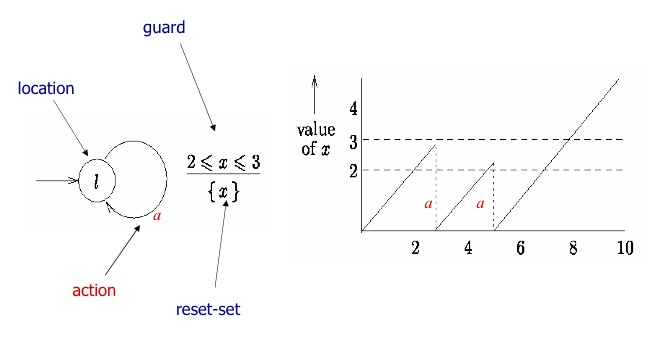
\includegraphics[width=8cm]{./images/model0.jpg} \\  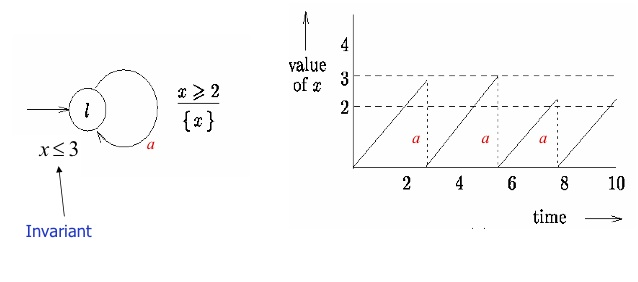
\includegraphics[width=7cm]{./images/model1.jpg}
\end{tabular}

\end{slide}

%----------------------------------------------------------------------------------
\begin{slide}{Transition guards \& location invariants}
\small

\begin{block}{Demo (in  \uppaal)}
~\\


\begin{tabular}{ccc}
  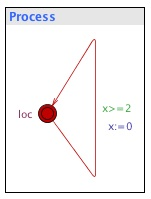
\includegraphics[width=3cm]{./images/g1.jpg} & 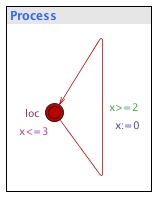
\includegraphics[width=3cm]{./images/g2.jpg} &  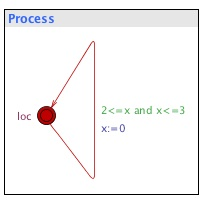
\includegraphics[width=3cm]{./images/g3.jpg}
\end{tabular}

\end{block}
\end{slide}


%----------------------------------------------------------------------------------
\begin{slide}{Parallel composition of timed automata}
\small

\begin{itemize}
\item Action labels as \structure{channel} identifiers
\item Communication by \structure{forced handshacking} over a subset of common actions
\item  Is defined as an automaton construction over a finite set of
  timed automata originating a so-called \dgold{network} of timed
  automata
\end{itemize}

\end{slide}

%----------------------------------------------------------------------------------
\begin{slide}{Parallel composition of timed automata}
\small

%\begin{block}{$TA_1 \parallel TA_2$}
Let $H \subseteq Act_1 \cap Act_2$. The parallel composition of $ta_1$ and  $ta_2$ synchronizing on $H$
is the timed automata
\begin{equation*}
\structure{ta_1 \parallel_H ta_2 := \pair{L_1 \times L_2, L_{0,1} \times L_{0,2}, Act_{\parallel_H}, C_1 \cup C_2, Tr_{\parallel_H}, Inv_{\parallel_H}}}
\end{equation*}
where
\begin{itemize}
\item $\structure{Act_{\parallel_H}} = ((Act_1 \cup Act_2) - H) \cup \enset{\tau}$
\item $\structure{Inv_{\parallel_H}} \pair{\ell_1,\ell_2} = Inv_1(\ell_1) \e  Inv_2(\ell_2)$
\item $\structure{Tr_{\parallel_H}}$ is given by:
\begin{itemize}
\item $\pair{\ell_1,\ell_2} \tran{g,a,U} \pair{\ell'_1,\ell_2}\; $ if $\; a \not \in H \e  \ell_1 \tran{g,a,U} \ell'_1 $
\item $\pair{\ell_1,\ell_2} \tran{g,a,U} \pair{\ell_1,\ell'_2}\; $ if $\; a \not \in H \e   \ell_2 \tran{g,a,U} \ell'_2$
\item $\pair{\ell_1,\ell_2} \tran{g,\tau,U} \pair{\ell'_1,\ell'_2}\; $ if $\; a \in H \e  \ell_1 \tran{g_1,a,U_1} \ell'_1 \e \ell_2 \tran{g_2,a,U_2} \ell'_2$\\
with $g = g_1 \e g_2$ and $U = U_1 \cup U_2$
\end{itemize}
\end{itemize}
%\end{block}
\end{slide}

%----------------------------------------------------------------------------------
\begin{slide}{Example: the lamp interrupt as a closed system}
\small

\medskip

\begin{columns}
\col{
  \centering    
  \uppbox[40mm]{Lamp}{./images/Lamp.pdf}\\[2mm]
  \uppbox[12mm]{User}{./images/User.pdf}
  % \includegraphics[width=8cm]{./images/lamp2.jpg}\\
  % 
\includegraphics[scale=0.1]{./images/User.pdf}\\
% \end{figure}

}
\col{
  \begin{block}{\uppaal:}
  \begin{itemize}
  \item takes $H = Act_1 \cap Act_2$ (actually as \structure{complementary} actions denoted by the \structure{?} and \structure{!} 
  annotations)
  \item  only deals with \structure{closed} systems 
  \end{itemize}
  \end{block}

  \doSimpleExercise{Define the TA of the composition.}
}
\end{columns}
\end{slide}

%----------------------------------------------------------------------------------
\begin{slide}{Exercise: worker, hammer, nail}
\small
\begin{columns}
\col[.45]{
  \centering
  ~\\[2mm]
  % Requires \usepackage{graphicx}
  % ~~~~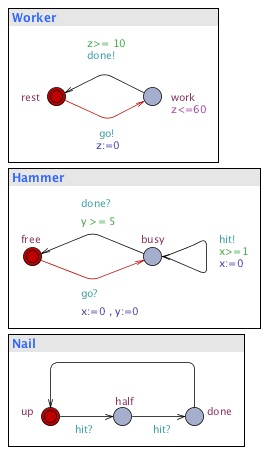
\includegraphics[width=45mm]{./images/WHN.jpg}
  \uppbox[30mm]{Worker}{./images/Worker.pdf}\\[2mm]
  \uppbox[30mm]{Hammer}{./images/Hammer.pdf}\\[2mm]
  \uppbox[30mm]{Nail}{./images/Nail.pdf}\\
}
\col[.54]{
  \doExercise[55mm]{Define the TA of the composition.}{}
}
\end{columns}
\end{slide}


\section{Semantics}


%----------------------------------------------------------------------------------
\begin{slide}{Timed Labelled Transition Systems}
\small\centering
\begin{tabular}{lc@{~~}l}
\toprule 
\alert{Syntax} && \alert{Semantics}\\
\cmidrule(lr){1-3}
\gry{\emph{How to write}} & & \gry{\emph{How to execute}}\\
Process Languages &  & LTS (Labelled Transition Systems)\\
\structure{Timed Automaton} &  & TLTS (Timed LTS) \\
\bottomrule
\end{tabular}
~\\
~\\
~\\
\pause

\begin{block}{Timed LTS}
Introduce \structure{delay transitions} to capture the passage of time within a LTS:
\begin{align*}
s \tran{a} s' & \;\; \text{for $a \in Act$, are ordinary transitions due to action occurrence }\\
s \tran{d} s' &\; \;  \text{for $d \in \R^+$, are \structure{delay} transitions}
\end{align*}
subject to a number of constraints, eg, 
\end{block}
\end{slide}


%----------------------------------------------------------------------------------
\begin{slide}{Dealing with time in system models}
\small
\begin{block}{Timed LTS}
\begin{itemize}
\item \structure{time additivity}
\begin{equation*}
(s \tran{d} s'  \e 0 \leq d' \leq d)\; \imp\; s  \tran{d'} s'' \tran{\; d-d'} s' \; \text{for some state $s''$}
\end{equation*}
\item delay transitions are \structure{deterministic}
\begin{equation*}
(s \tran{d} s'  \e s \tran{d} s'')\; \imp\; s'  = s''
\end{equation*}
%\item a state can only reach itself \structure{without delay}
%\begin{equation*}
%s \tran{0} s  \; \text{for all states $s$}
%\end{equation*}
\end{itemize}
\end{block}
\end{slide}







%----------------------------------------------------------------------------------
\begin{slide}{Semantics of Timed Automata}
\small

\begin{block}{Semantics of TA:}
Every TA $ta$ defines a TLTS 
\begin{equation*}
\structure{\TL{ta}}
\end{equation*}
whose states are pairs 
\begin{equation*}
\pair{\structure{\text{location}}, \structure{\text{clock valuation}} }
\end{equation*}
with \structure{infinitely}, even \structure{uncountably} many states, and infinite branching
\end{block}
\end{slide}

%----------------------------------------------------------------------------------
\begin{slide}{Clock valuations}
\small


\begin{block}{Definition}
A \structure{clock valuation} \alert{$\eta$} for a set of clocks $C$ is a function 
\begin{equation*}
\fdec{\alert{\eta}}{C}{\R_0^+}
\end{equation*}
assigning to each clock $x \in C$ its current value $\alert{\eta}\, x$.
\end{block}
~\\

\begin{block}{Satisfaction of clock constraints}
\begin{align*}
\alert{\eta} \models x \mathbin{\square} n \; & \dimp\; \alert{\eta}\, x \mathbin{\square} n\\
\alert{\eta} \models x-y \mathbin{\square} n \; & \dimp\; (\alert{\eta}\, x - \alert{\eta}\, y) \mathbin{\square} n\\
\alert{\eta} \models g_1 \e g_2 \; & \dimp\; \alert{\eta} \models g_1 \e \alert{\eta} \models g_2
\end{align*}
\end{block}
\end{slide}

%----------------------------------------------------------------------------------
\begin{slide}{Operations on clock valuations}
\small


\begin{block}{Delay}
For each $d \in \R_0^+$, valuation $\eta \alert{+ d}$ is given by
\begin{equation*}
(\eta \alert{+ d})\, x\; =\; \eta\, x\; +\; d
\end{equation*}
\end{block}
~\\

\begin{block}{Reset}
For each $R \subseteq C$, valuation $\eta\alert{[R]}$ is given by
\begin{equation*}
\begin{cases}
\eta\alert{[R]}\, x\; =\; \eta\, x & \; \rimp\; x \not\in R\\
\eta\alert{[R]}\, x\; =\; 0 & \; \rimp\; x \in R
\end{cases}
\end{equation*}
\end{block}
\end{slide}

%----------------------------------------------------------------------------------
\begin{slide}{From $ta$ to $\TL{ta}$}
\small
Let $ta = \pair{L, L_0, Act, C, Tr, Inv}$
\begin{equation*}
 \structure{\TL{ta}\; =\; \pair{S, S_0 \subseteq S, N, T}}
\end{equation*}
where
\begin{itemize}
\item $S = \setdef{\pair{l,\alert{\eta}} \in  L \times \alert{(\R_0^+)^C}}{\alert{\eta} \models Inv(l)}$
\item $S_0 = \setdef{\pair{\ell_0,\alert{\eta}}}{\ell_0 \in L_0\; \e\;  \alert{\eta}\, x = 0\; \text{for all $x \in C$}}$
\item $N = Act \cup \alert{\R_0^+}$ (ie, \alert{transitions can be labelled by actions or delays})
\item $T \subseteq S \times N \times S$ is given by:
\end{itemize}
\begin{align*}
\pair{l,\alert{\eta}} \tran{a} \pair{l',\alert{\eta'}}\; & ~~\rimp~~\; 
\exists_{l \tran{g,a,U} l' \in Tr}  \; \;\alert{\eta} \models g \; \e\; \alert{\eta'} = \alert{\eta}[U] \; \e\;  \alert{\eta'} \models Inv(l')\\
\pair{l,\alert{\eta}} \tran{\alert{d}} \pair{l,\alert{\eta +d}}\; & ~~\rimp~~\; 
\exists_{\alert{d \in \R_0^+}}  \; \;  \alert{\eta + d} \models Inv(l)
\end{align*}
\end{slide}

%----------------------------------------------------------------------------------
\begin{slide}{Example: the simple switch}
\small
\begin{figure}[htb]
  \centering
  % \includegraphics[width=5cm]{./images/PASswitchA.jpg}\\
  \uppbox[5cm]{Switch}{./images/SwitchA}\\
\end{figure}

\doExercise{Define $\TL{\mathsf{SwitchA}}$}{
\begin{equation*}
S = \pause \setdef{\pair{off,\overline t}}{t \in \R_0^+} \cup \setdef{\pair{on,\overline t}}{0 \leq t \leq 2} 
\end{equation*}
where $\overline{t}$ is a shorthand for $\eta$ such that $\eta\, x = t$
}
\exerciseBack

\end{slide}

%----------------------------------------------------------------------------------
\begin{slide}{Example: the simple switch}
\small
\begin{figure}[htb]
  \centering
  % \includegraphics[width=5cm]{./images/PASswitchA.jpg}\\
  \uppbox[5cm]{Switch}{./images/SwitchA}\\
\end{figure}

\doExercise{Define $\TL{\mathsf{SwitchA}}$}{
\vspace{-7mm}
\begin{align*}
\only<1>{T = \ldots}
\uncover<2->{
\pair{off,\overline t} \tran{d} \pair{off,\overline t+d}\; & \; \text{for all $t,d \geq 0$}\\
 \pair{off,\overline t} \tran{in} \pair{on,\overline 0}\; & \; \text{for all $t \geq 0$}\\
\pair{on,\overline t} \tran{d} \pair{on,\overline t+d}\; & \; \text{for all $t,d \geq 0$ and $t+d \leq 2$}\\
\pair{on,\overline t} \ \tran{out} \pair{off,\overline t}\; & \; \text{for all $1 \leq t \leq 2$}
}
\end{align*}
}
\exerciseBack
\end{slide}
\exerciseAdd

%----------------------------------------------------------------------------------
\begin{slide}{Note}
\small

\begin{itemize}
\item The elapse of time in timed automata \structure{only} takes place in locations:
\item ... actions take place instantaneously 
\item Thus, several actions may take place at a single time unit
\end{itemize}
\end{slide}

%----------------------------------------------------------------------------------
\begin{slide}{Behaviours}
\small

\begin{itemize}
\item Paths in $\TL{ta}$ are \structure{discrete representations of continuous-time behaviours} in $ta$
\item ... at least they indicate the states immediately before and after the execution of an action
%\item Such paths can also be represented graphically through \structure{location diagrams}
\item However, as interval delays may be realised in \alert{uncountably} many different ways, different paths 
may represent the same behaviour
\pause
\item ... but not all paths correspond to valid  (\structure{realistic}) behaviours:
\end{itemize}

\begin{block}{undesirable paths:}
\begin{itemize}
\item  \structure{time-convergent} paths
\item  \structure{timelock} paths
\item  \structure{zeno} paths
\end{itemize}
\end{block}
\end{slide}

%----------------------------------------------------------------------------------
\begin{slide}{Time-convergent paths}
\small

\begin{equation*}
\pair{l,\eta}  \tran{d_1} \pair{l,\eta + d_1}  \tran{d_2} \pair{l,\eta + d_1 + d_2}  \tran{d_3} \pair{l,\eta + d_1 + d_2 + d_3}  \tran{d_4} 
\cdots  
\end{equation*}
such that 
\begin{equation*}
\forall_{i \in N}\st\, d_i > 0\; \e\; \sum_{i \in N}  d_i = d
\end{equation*}
ie, the \alert{infinite sequence of delays converges toward $d$}

\begin{itemize}
\item Time-convergent path are \alert{conterintuitive}; as their existence cannot be avoided, they are simply  \structure{ignored} in the semantics of Timed Automata
\item Time-\structure{divergent} paths are the ones in which time always progresses
\end{itemize}
\end{slide}

%----------------------------------------------------------------------------------
\begin{slide}{Time-convergent paths}
\small

\begin{block}{Definition}
An infinite path fragment $\rho$ is \structure{time-divergent} if $\ET{\rho} = \infty$\\
Otherwise is  \structure{time-convergent}. 
\end{block}

where
\begin{align*}
\ET{\rho}\; & =\; \sum_{i=0 .. \infty} \ET{\delta}\\
\ET{\delta}\; & =\; \begin{cases}
0 & \rimp\;  \delta \in Act\\
\delta & \rimp\:  \delta \in \R_0^+
\end{cases}
\end{align*}
for $\rho$ a path and $\delta$ a label in $\TL{ta}$ 
\end{slide}

%----------------------------------------------------------------------------------
\begin{slide}{Timelock paths}
\small

\begin{block}{Definition}
A path is \structure{timelock} if it contains a state with a timelock, ie, a \alert{state
from which there is not any time-divergent path}
\vspace{0.3cm}

A \structure{timelock} represents a situation that causes time progress to halt (e.g. when it is impossible to leave a location before its invariant becomes invalid)
\end{block}

\begin{itemize}
\item any \structure{teminal state} ($\neq$ terminal location) in $\TL{ta}$ contains a timelock
\item ... but not all timelocks arise as terminal states in $\TL{ta}$
\end{itemize}
\end{slide}



%----------------------------------------------------------------------------------
\begin{slide}{Timelock paths}
\small

\begin{center}
  % 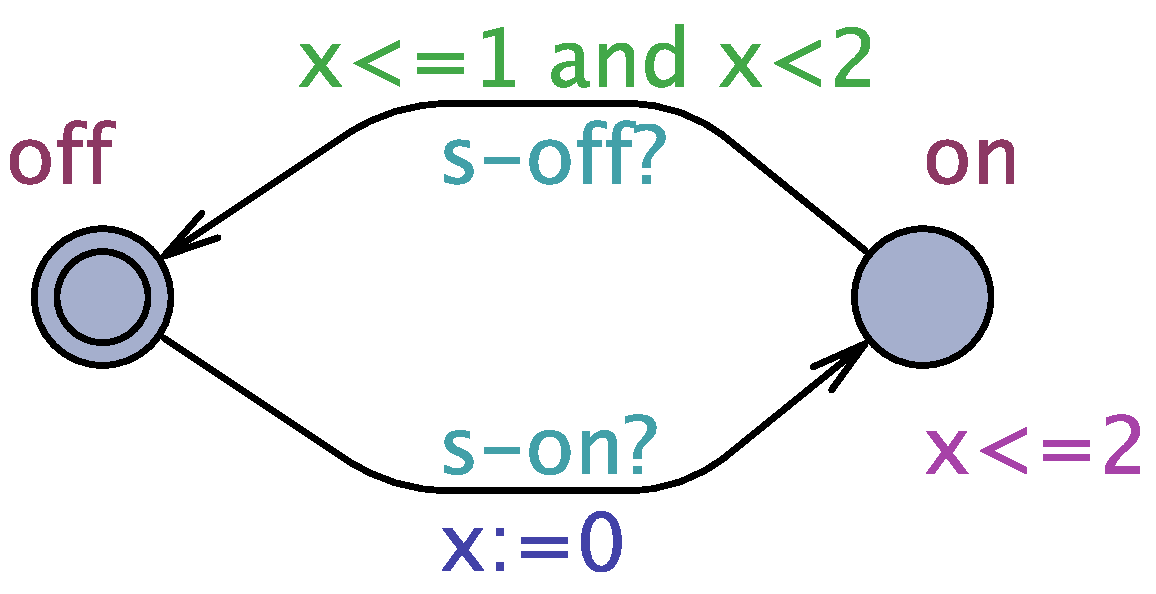
\includegraphics[width=4.5cm]{./images/SwitchB} 
  \uppbox[4.5cm]{NoTimelock}{./images/SwitchB} 
\end{center}

State $\pair{on,2}$ is reachable through path 
$$\pair{off,0} \tran{s-on} \pair{on,0} \tran{2} \pair{on,2}$$
and is terminal

\end{slide}

%----------------------------------------------------------------------------------
\begin{slide}{Timelock paths}
\small


\begin{center}
  % 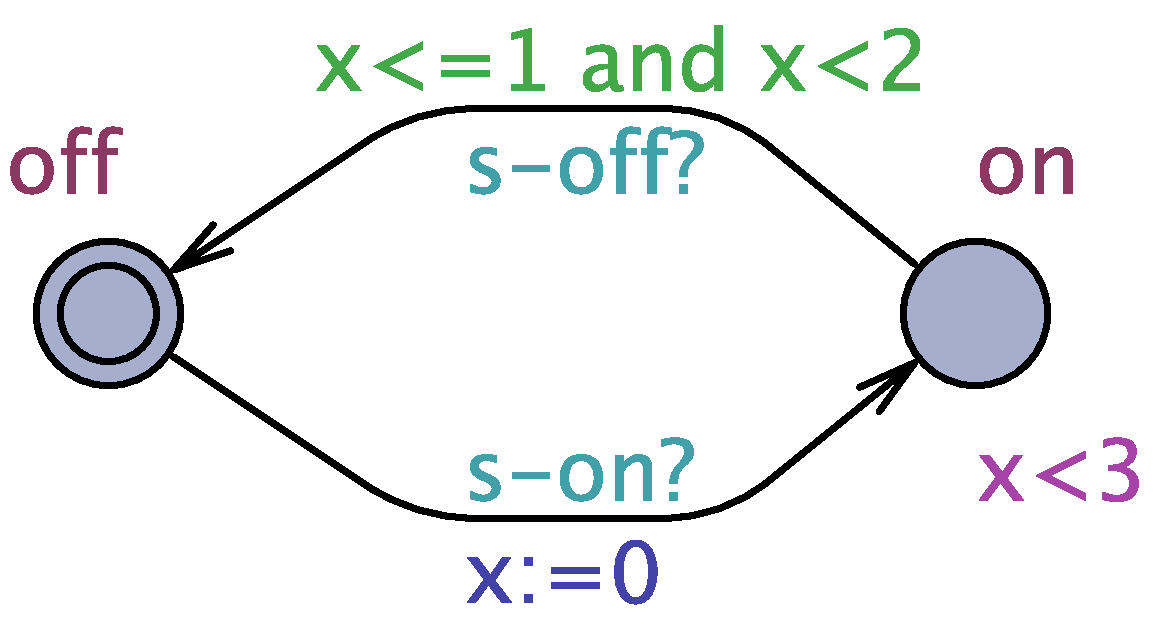
\includegraphics[width=4.5cm]{./images/SwitchC} 
  \uppbox[4.5cm]{Timelock}{./images/SwitchC} 
\end{center}

State $\pair{on,2}$ is not terminal but has a \structure{convergent} path:

$$\pair{on,2} \pair{on,2.9}  \pair{on,2.99}  \pair{on,2.999}  ...$$

\end{slide}



%----------------------------------------------------------------------------------
\begin{slide}{Zeno}
\small

\begin{block}{In a Timed Automaton}
\begin{itemize}
\item The elapse of time only takes place at \structure{locations}
\item Actions occur \structure{instantaneously}: at a single time instant several actions may take place
\end{itemize}

\caixa{... it may perform \structure{infinitely} many actions in a \structure{finite} time interval \\
(non realizable because it would require infinitely fast processors)}
\end{block}

\pause
\begin{block}{Definition}
An infinite path fragment $\rho$ is \structure{zeno} if it is \alert{time-convergent} and
\alert{infinitely many actions occur along it}



A timed automaton $ta$ is \structure{non-zeno} if there is not an initial zeno path in $\TL{ta}$
\end{block}

\end{slide}


%----------------------------------------------------------------------------------
\begin{slide}{Zeno}
\small


\begin{block}{Example}
Suppose the user can press the $in$ button when the light is $on$ in
\begin{figure}[htb]
  \centering
  % \includegraphics[width=5cm]{./images/PASswitchD.jpg}\\
  \uppbox[5cm]{Zeno}{./images/SwitchD}\\
\end{figure}
In doing so clock $x$ is reset to 0 and light stays $on$ for more 2 time units (unless the button is pushed again ...)
\end{block}

\end{slide}

%----------------------------------------------------------------------------------
\begin{slide}{Zeno}
\small


\begin{block}{Example}
\alert{Typical paths:}
The user presses $in$ \alert{infinitely fast}:
\begin{equation*}
\pair{off,0}  \tran{in}  \pair{on,0}  \tran{in}  \pair{on,0}  \tran{in}  \pair{on,0}  \tran{in}  \pair{on,0}  \tran{in} \cdots
\end{equation*}


The user presses $in$ \alert{faster and faster}:
\begin{equation*}
\pair{off,0}  \tran{in}   \pair{on,0}  \tran{0.5} \pair{on,0.5} \tran{in} \pair{on,0} \tran{0.25}  \pair{on,0.25}   \tran{in} \pair{on,0}  \tran{0.125}  \cdots
\end{equation*}
\end{block}

\caixa{How can this be fixed?}

\myblock{Time shall pass!}

\end{slide}


%----------------------------------------------------------------------------------
\begin{slide}{Zeno}
\small


\begin{block}{Sufficient criterion for nonzenoness}
A timed automaton is nonzeno if on any of its control cycles time advances with at least some  
\structure{constant amount} ($\geq 0$). Formally, if for every control cycle
\begin{equation*}
{\red \ell_0} \tran{g_0, a_0, U_0} \ell_1 \tran{g_1, a_1, U_1} \cdots  \tran{g_n, a_n, U_n} {\red \ell_0} 
\end{equation*}
there exists a clock $x \in C$ such that
\begin{enumerate}
\item  $x \in U_i$ (for $0 \leq i \leq n$)
\item for all clock valuations \structure{$\eta$}, there is a  $\structure{c} \in \N_{>0}$ such that
\begin{equation*}
\structure{\eta}(x) < \structure{c}\; \imp\; ((\eta \not\models g_j)\; \ou\; \lnot Inv(\ell_j)) \; \text{for some $0 \leq j \leq n$}
\end{equation*}
\end{enumerate}


\end{block}

\end{slide}


%----------------------------------------------------------------------------------
\begin{slide}{Warning}
\small

Both 
\begin{itemize}
\item timelocks
\item zenoness
\end{itemize}
are \structure{modelling flaws} and need to be avoided.


\begin{block}{Example}
In the example above, it is enough to impose a non zero minimal delay  between successive button pushings.
\end{block}

\end{slide}




\section{Modelling in \uppaal}
%----------------------------------------------------------------------------------
\begin{slide}{\uppaal}
\small

... an \structure{editor},  \structure{simulator} and \structure{model-checker} for TA with \structure{extensions} ...

\structure{Editor.}
\vspace*{-3mm}
\begin{itemize}
\item \alert{Templates} and \alert{instantiations}
\item Global and local \alert{declarations}
\item \alert{System definition}
\end{itemize}

\structure{Simulator.}
\vspace*{-3mm}
\begin{itemize}
\item Viewers: \alert{automata animator} and \alert{message sequence chart}
\item Control (eg, \alert{trace} management)
\item Variable view: shows values of the integer variables and the clock constraints defining symbolic states
\end{itemize}

\structure{Verifier.}
\vspace*{-3mm}
\begin{itemize}
\item (\texttt{see next session)}
\end{itemize}

\end{slide}


%----------------------------------------------------------------------------------
\begin{slide}{Extensions (modelling view)}
\small

\begin{itemize}
\item \structure{templates} with \alert{parameters} and an \alert{instantiation mechanism}
\item \structure{data expressions} over \structure{bounded integer variables} (eg, \texttt{int[2..45] x}) allowed in \alert{guards},
\alert{assigments} and \alert{invariants}
\item rich set of \structure{operators} over integer and booleans, including bitwise operations, arrays, initializers ... in general
a whole \structure{subset of C} is available
\item \structure{non-standard} types of \alert{synchronization}
 \item \structure{non-standard} types of \alert{locations}
\end{itemize}
\end{slide}




%----------------------------------------------------------------------------------
\begin{slide}{Extension: broadcast synchronization}
\small



\begin{itemize}
\item A sender  can synchronize with an arbitrary number of receivers 
\item Any receiver than can synchronize in the current state must do so
\item Broadcast sending is never blocking (the send action can occur even with no receivers).
\end{itemize}

\end{slide}

%----------------------------------------------------------------------------------
\begin{slide}{Extension: urgent synchronization}
\small

\begin{columns}
  \column{0.3\textwidth}
     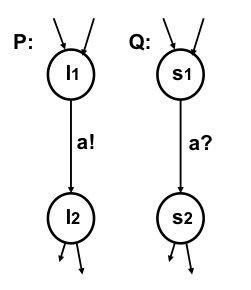
\includegraphics[width=\textwidth]{./images/urgent.jpg} 

  \column{0.7\textwidth}
    Channel $a$ is declared \structure{\texttt{urgent chan a}} if both edges are to be taken as soon as they are ready 
    (\alert{simultaneously} in locations $\ell_1$ and $s_1$).

    Note the problem can  \alert{not} be solved with \alert{invariants} because locations $\ell_1$ and $s_1$ 
    can be reached at different moments

    \begin{itemize}
    %\item Declare as \texttt{urgent chan a}
    \item No delay allowed if a synchronization transition on an urgent channel is enabled
    \item Edges using urgent channels for synchronization cannot have time constraints (ie, clock guards)
    \end{itemize}
\end{columns}
\end{slide}


%----------------------------------------------------------------------------------
\begin{slide}{Extension: urgent location}
\small

\begin{columns}
  \column{0.3\textwidth}
     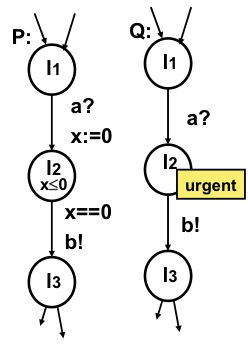
\includegraphics[width=\textwidth]{./images/urgent2.jpg} 

  \column{0.7\textwidth}
    \begin{itemize}
    %\item Declare as \texttt{urgent chan a}
    \item Time does not progress but interleaving with normal location is allowed
    \item Both models are equivalent: \alert{no delay at an urgent location}
    \item but the use of \structure{urgent location} reduces the number of clocks in a model and simplifies analysis
    \end{itemize}
\end{columns}

\end{slide}


%----------------------------------------------------------------------------------
\begin{slide}{Extension: committed location}
\small\centering

% \begin{itemize}
% \end{itemize} 

\begin{columns}
\column{0.3\textwidth}
   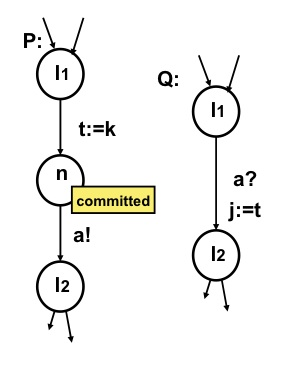
\includegraphics[width=\textwidth]{./images/urgent1.jpg} 

\column{0.7\textwidth}
\begin{itemize}
\item delay is not allowed and the committed transition must be left in the next instant (or one of them if there are several), i.e., 
next transition must involve an outgoing edge of at least one of the committed locations
\item Our aim is to pass the value $k$ to variable $j$ (via global variable $t$)
\item Location $n$ is \structure{committed} to ensure that no other automata can assign $j$ before
the assignment $j:=t$
\end{itemize}
\end{columns}


\end{slide}

%%----------------------------------------------------------------------------------
%\begin{slide}{Modelling patterns: Value passing}
%\small
%
%\begin{center}
% \includegraphics[width=10cm]{pass.jpg} 
%\end{center}
%\end{slide}
%
%%----------------------------------------------------------------------------------
%\begin{slide}{Hints}
%\small
%
%
%\begin{itemize}
%\item \alert{Modelling patterns}: see the \uppaal\ tutorial
%\item \alert{Further examples}: see the \texttt{demo} folder in the standard distribution
%\end{itemize}
%
%\end{slide}
%
%%----------------------------------------------------------------------------------
%----------------------------------------------------------------------------------
\begin{slide}{The train gate example}
\small
\begin{columns}

\begin{column}{5cm}
\begin{center}
% \includegraphics[width=5cm]{./images/tg1.jpg} 
\uppbox[5cm]{Train(id)}{./images/Train}
\end{center}
\end{column}

\col[0.65]{
\begin{itemize}
\item Events model approach/leave, order to stop/go
\item A train can not be stopped or restart instantly
\item After approaching  it has 10m to receive a stop. 
\item After that it  takes further 10 time units to reach the bridge
\item After restarting takes 7 to 15m to reach the cross and 3-5 to cross
\end{itemize}
}
\end{columns}
\end{slide}


%----------------------------------------------------------------------------------
\begin{slide}{The train gate example}
\small

\begin{center}
% \includegraphics[width=5cm]{./images/tg2.jpg} 
\uppbox[5cm]{Gate}{./images/Gate}
\end{center}

\begin{itemize}
\item Note the use of parameters and the select clause on transitions
\item Programming ...
\end{itemize}

\end{slide}

%\begin{frame}[fragile]{Fisher's mutual exclusion protocol}
%\small
%
%\begin{columns}
%\column{.4\textwidth}
%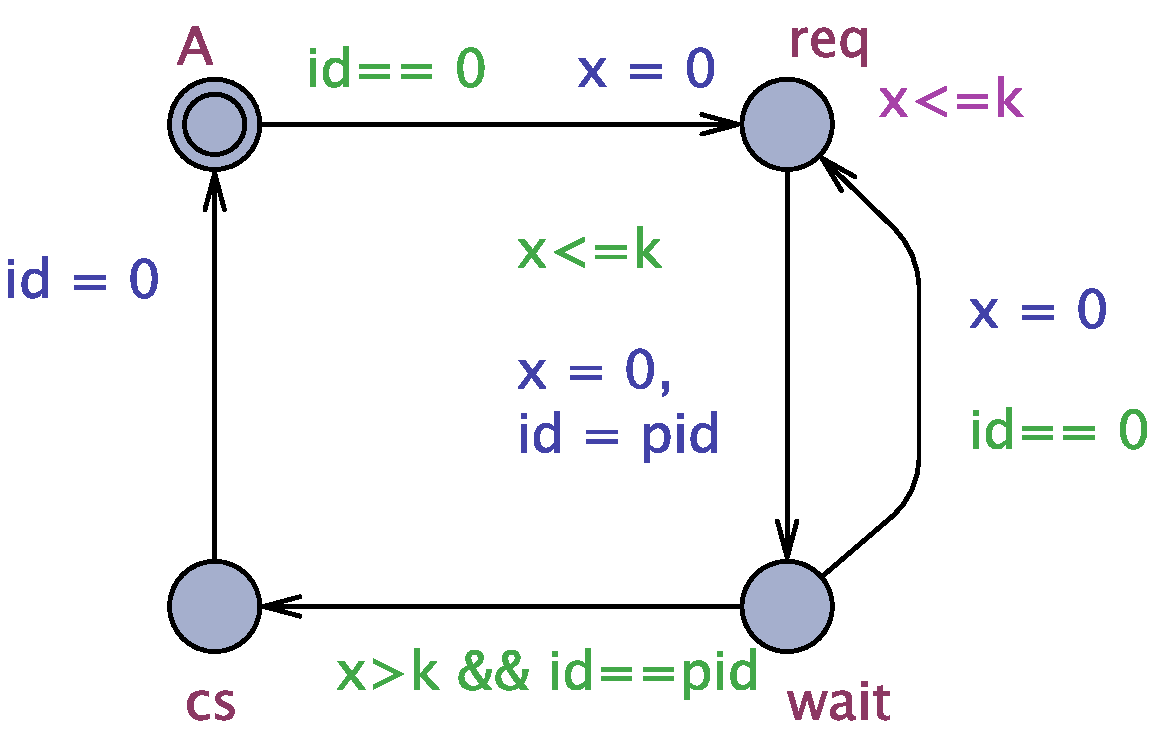
\includegraphics[width=1.1\textwidth]{./images/P.pdf} 
%
%\column{.58\textwidth}
%\begin{itemize}
%  \item Processes want to access a shared Critical Section
%  \item Send a request for the access
%  \item Wait $k$ time units -- if access is not given, resend a request
%\end{itemize}
%\end{columns}
%
%\bigskip
%
%\begin{lstlisting}[emph={[2]forall}]
%% P(1) requests access => it will eventually wait
%P(1).req -> P(1).wait
%% mutual exclusion invariant
%A[] forall (i:int[1,6]) forall (j:int[1,6])
%  P(i).cs && P(j).cs imply i == j  
%\end{lstlisting}
%
%\end{frame}



%%%%%%%%%%%%%%%%%%%%%%%%%%

\end{document}
